\subsection{EMG-forstærker}

EMG-forstærkeren testes for at vurdere, hvorvidt muskelsignalerne fra rectus femoris opsamles. Overfladeelektroderne placeres midt for linjen mellem anterior spina iliaca superior og den superiore del af patella ud fra SENIAM's anvisning om elektrodeplacering \citep{seniam2016}. En squat-øvelse udføres, mens muskelsignaler opsamles i MATLAB. Muskelsignalet som en energirepræsentation under udførslen af squat-øvelsen fremgår af \autoref{fig:raat_emg}. 

\begin{figure}[H]
\centering
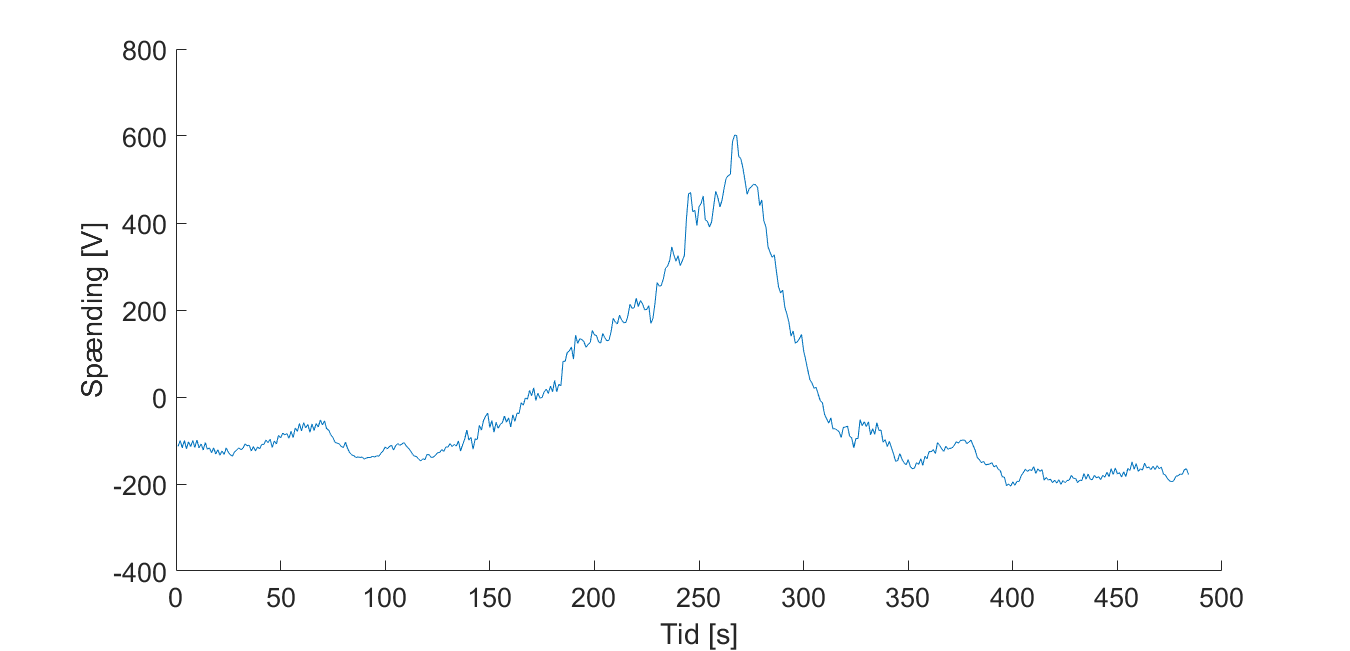
\includegraphics[width=0.8\textwidth]{figures/raat_EMG_test}
\caption{Et ufiltreret EMG-signal fra rectus femoris under udførsel af en squat-øvelse}
\label{fig:raat_emg}
\end{figure}

Opsamlingen skete med en spændingsforsyning på $\pm5,5~V$, og på EMG-forstærkeren findes et justerbart gain, så forstærkningen kan tilpasses den enkelte bruger af systemet. Ud fra dette og \autoref{fig:raat_emg} vurderes det, at EMG-forstærkeren opfylder de opstillede krav i \autoref{EMG_krav}

\subsection{Accelerometre}

Accelerometrene testes for at vurdere, hvorvidt de opstillede krav i \autoref{sec:acc_teori_krav} opfyldes. Der tages udgangspunkt i værdierne fra databladet for ADXL335 \citep{analogdevices2010}, da det ikke er muligt at teste alle opstillede krav. Databladet oplyser, at de kan forsynes med en DC-forsyning fra $1,8-3,6~V$. Da accelerometrene skal kunne forsynes med en spænding på $3,3~V$, opfyldes dette krav. Herudover ses det ud fra databladet, at der er en linearitet med en afvigelse på $0,3\%$ samt et lineært arbejdsområde på $ \pm 3 g$. Af databladet fremgår det ligeledes, at accelerometrene er triaksiale. Det er derfor muligt at måle på minimum én akse, hvilket er det opstillede krav. Af denne grund er opfylder accelerometrene kravene.  

